\documentclass[aspectratio=169]{beamer}

\usetheme[progressbar=frametitle]{metropolis}
\usepackage{appendixnumberbeamer}

\usepackage{booktabs}
\usepackage[scale=2]{ccicons}

\usepackage{pgfplots}
\usepgfplotslibrary{dateplot}

\usepackage{amssymb}
\usepackage{amsmath}
\usepackage{amsthm}
\usepackage{mathabx}

\usepackage{float}
\setlength{\leftmargini}{0pt}

\usepackage{bbm}
\usepackage{pgf, tikz}
\usetikzlibrary{positioning}
\usepackage{tcolorbox}

\newtheorem*{assumption}{Assumption}

\usepackage{xspace}
\newcommand{\themename}{\textbf{\textsc{metropolis}}\xspace}
\DeclareMathOperator*{\E}{\mathbb{E}}
\DeclareMathOperator*{\R}{\mathbb{R}}
\DeclareMathOperator*{\Var}{\mathbb{V}ar}
\DeclareMathOperator{\fa}{\hspace{.1cm} \forall \hspace{.1cm}}
\newcommand{\wh}{\widehat}
\newcommand{\wtl}{\widetilde}
\def\argmin{\mathop{\textrm{argmin}}}
\def\1{\mathop{\mathbbm 1}\nolimits}
\newcommand{\Ex}{{\mathbb E}}
\newcommand{\PP}{\mathbb{P}}

\setbeamertemplate{theorems}[numbered] 
\newtheorem*{remark}{Remark} 
\newtheorem*{defin}{Definition}
\newtheorem*{thm}{Theorem}
\newtheorem*{ex}{Example}

\makeatother

\title{How Acquisitions Affect Firm Behavior and Performance: Evidence from the Dialysis Industry}
\subtitle{Paul J. Eliason et al.}

\date{November 23, 2022}
\author{Jung Jae Kim}

\begin{document}
\lecture{Test lecture one}{lone}

\maketitle
%Start of the document

\begin{frame}{Motivation}

\begin{itemize}
\item Concentration through mergers and acquisitions 
    \begin{itemize}
        \item Lower costs and better patient outcomes vs. Higher prices and lower quality
    \end{itemize}
\item Literature has focused on how mergers affect prices through change in market power.
\item Less work has examined the precise channels through which mergers lead to changes in outcomes.
\end{itemize}

\begin{itemize}
    \item[] \textbf{Research objective}: How large chains transfer their corporate strategies to the independent facilities they acquire in U.S. dialysis industry.
    \begin{itemize}
        \item Dialysis is a fairly standardized treatment that allows for a direct comparison.
        \item The dialysis industry has become increasingly concentrated: Two largest corporations, DaVita and Fresenius, own more than 60\% of facilities.
    \end{itemize}
\end{itemize}

\end{frame}

\begin{frame}{U.S. Dialysis Industry}

\begin{itemize}
\item Dialysis: a medical procedure that cleans blood of patients suffering from end-stage renal disease (ESRD).
\item Although a kidney transplant is considered the best treatment, it is often not possible.
\item In addition to dialysis, most ESRD patients receive treatment for anemia.
\item Anemia is treated with a cocktail of injectable drugs, EPOGEN (EPO), along with an iron analog, such as Venofer or Ferrlecit.
\item A dialysis facility's quality measure: clinical indicator and patient outcomes.
    \begin{itemize}
        \item [(1)] Urea reduction ratio (URR) and hemoglobin (Hgb) levels.
        \item [(2)] Mortality and hospitalization.
    \end{itemize}

\end{itemize}

\end{frame}

\begin{frame}{U.S. Dialysis Industry}

\begin{itemize}
\item All ESRD patients become eligible for Medicare coverage, regardless of age.
\item Medicare paid a composite rate of \$128 per dialysis, up to 3 times a week.
\item For injectable drugs, providers were reimbursed separately on a fee-for-service basis depending on the quantity of drug administered.
\item Administering EPO proved lucrative for providers, accounting for 25\% of DaVita's revenue.
\item Venofer and Ferrlecit are substitutable, but facilities could effectively receive higher reimbursements per vial for Venofer.


\end{itemize}

\end{frame}

\begin{frame}{Preview of the Main Results}

\begin{itemize}
\item Acquired facilities alter their treatments in ways that increase reimbursement and decrease costs.
    \begin{itemize}
        \item [(1)] Patients' EPO doses increase 129\% at independent facilities acquired by large chains.
        \item [(2)] The facilities increase use of Venofer relative to Ferrlecit that offers lower reimbursements.
        \item [(3)] Large chains replace high-skill nurses with lower-skill technicians at the facilities.
        \item [(4)] Facilities increase the patient load of each employee by 11.7\% and increase the number of patients by 4.5\%, potentially reducing the quality of care.
    \end{itemize}
\item Patients at acquired facilities are 4.2\% more likely to be hospitalized in a given month.
\item Survival rate for new patients fall by 1.3-2.9\%.
\item New ESRD patients are 8.5\% less likely to receive a kidney transplant.
\item Patients are 5.1\% less likely to have Hgb levels within the recommended range.
\item Patients become 1.8\% more likely to have adequate URR.
\end{itemize}

\end{frame}

\begin{frame}{Data}
\begin{itemize}
\item Patient- and facility-level data from the United States Renal Data System (USRDS).
\item Treatment history for almost all dialysis patients since 1991.
\item Detailed data on dialysis facilities come from the Annual Facility Survey.
\end{itemize}

\end{frame}

\begin{frame}\frametitle{Summary Statistics}
 \begin{figure}[h!]
        \centering
        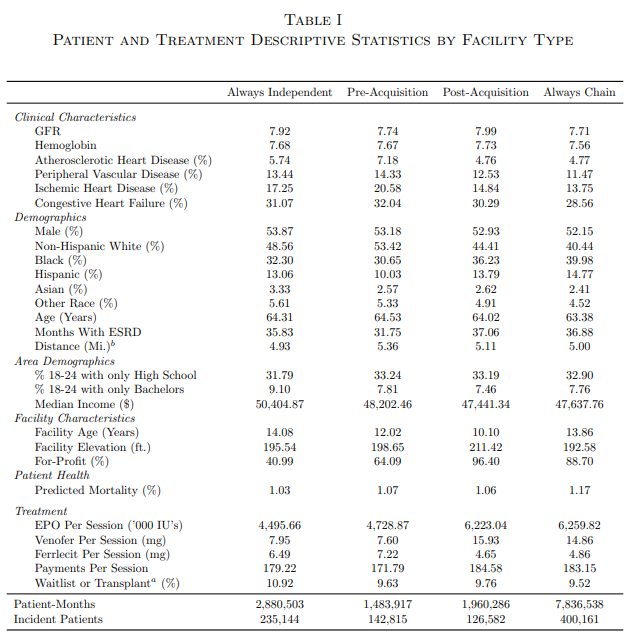
\includegraphics[width=75mm]{figure3_5.png}
        \label{fig:method}
        \end{figure}
\end{frame}


\begin{frame}{Empirical Models}
\begin{itemize}
\item[A.] \textit{Patient-Level Analysis}
\begin{equation}
Y_{i j t}=\beta^{\text {Pre }} D_{j t}^{\text {Pre }}+\beta^{\text {Post }} D_{j t}^{\text {Post }}+\beta^{\text {Chain }} D_{j t}^{\text {Chain }}+\alpha X_{i j t}+\epsilon_{i j t}
\end{equation}
             \begin{align*}
                Y_{ijt}&: \; \text{outcome of interest for patient $i$ at facility $j$ in month $t$}\\
                X_{ijt}&: \; \text{facility and patient controls \& year, month, and facility fixed effects}
            \end{align*}
\item  Note that when including facility fixed effects, $\beta^{\text {Pre }}$ and $\beta^{\text {Chain }}$ are absorbed.
\end{itemize}

\end{frame}

\begin{frame}\frametitle{Result: Drug Doses}
\setlength{\leftmargini}{12pt}
\vspace{-7.5mm}
 \begin{figure}[h!]
        \centering
        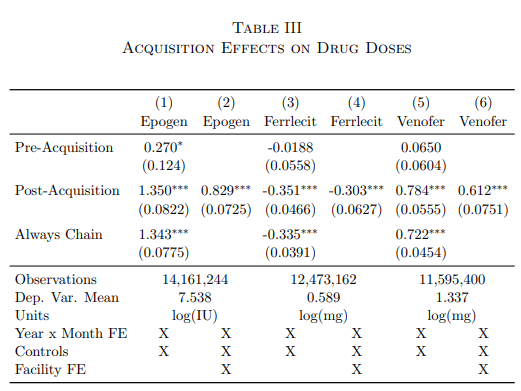
\includegraphics[width=95mm]{figure3_1.png}
        \label{fig:method}
        \end{figure}
        \vspace{-9.5mm}

\end{frame}

\begin{frame}\frametitle{Result: Drug Doses}
\setlength{\leftmargini}{12pt}
\vspace{-7.5mm}
 \begin{figure}[h!]
        \centering
        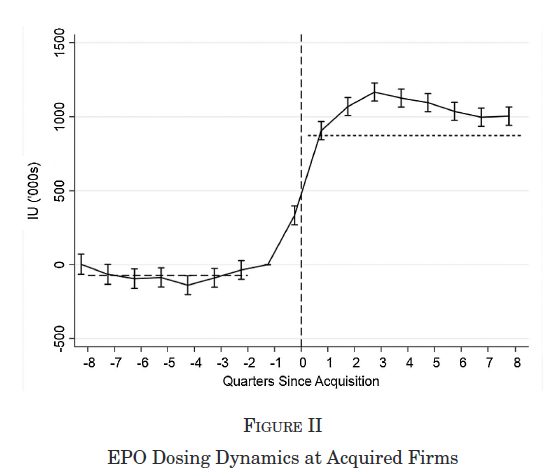
\includegraphics[width=85mm]{figure3_6.png}
        \label{fig:method}
        \end{figure}
        \vspace{-9.5mm}

\end{frame}

\begin{frame}{Empirical Models}
\begin{itemize}
\item[B.] \textit{Facility-Level Analysis}
\begin{equation}
Y_{j t}=\gamma^{\text {Post }} D_{j t}^{\text {Post }}+\delta X_{j t}+\nu_{j t}
\end{equation}
             \begin{align*}
                Y_{ijt}&: \; \text{outcome of interest for facility $j$ in month $t$}\\
                X_{ijt}&: \; \text{facility controls \& year and facility fixed effects}
            \end{align*}
\end{itemize}

\end{frame}

\begin{frame}\frametitle{Result: Facility Input Choices}
\setlength{\leftmargini}{12pt}
\vspace{-7.5mm}
 \begin{figure}[h!]
        \centering
        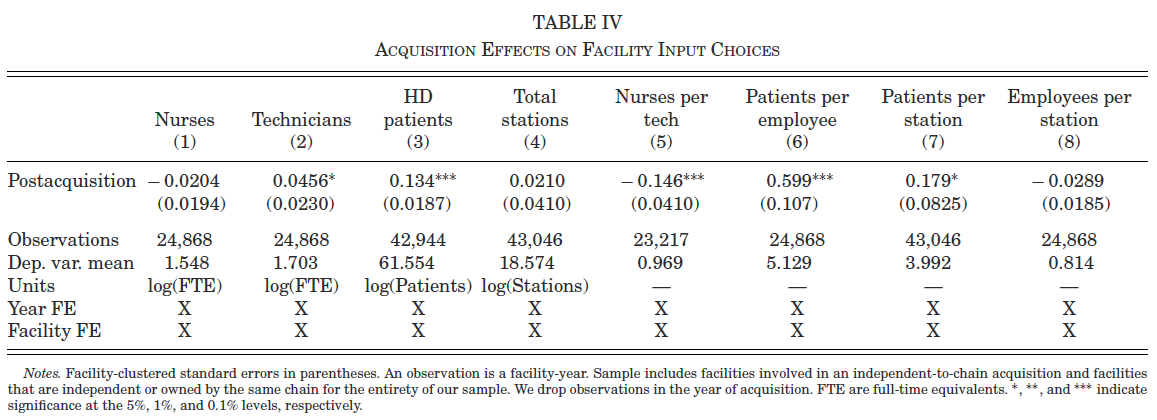
\includegraphics[width=140mm]{figure3_2.png}
        \label{fig:method}
        \end{figure}
        \vspace{-9.5mm}

\end{frame}

\begin{frame}\frametitle{Result: Patient Outcomes}
\setlength{\leftmargini}{12pt}
\vspace{-7.5mm}
 \begin{figure}[h!]
        \centering
        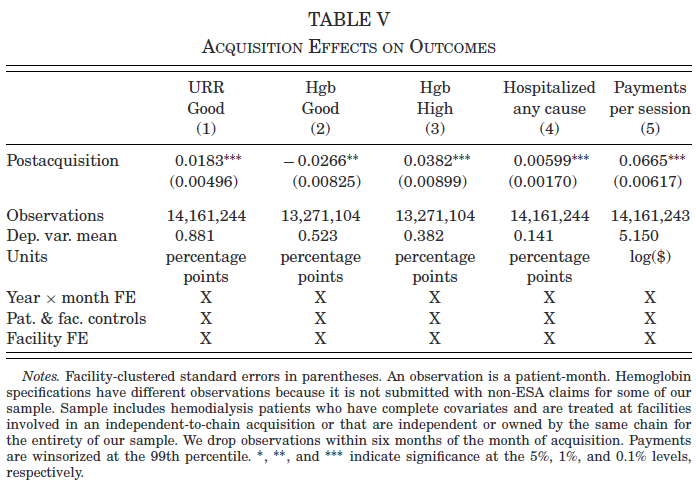
\includegraphics[width=100mm]{figure3_3.png}
        \label{fig:method}
        \end{figure}
        \vspace{-9.5mm}

\end{frame}

\begin{frame}\frametitle{Result: Patient Outcomes}
\setlength{\leftmargini}{12pt}
\vspace{-7.5mm}
 \begin{figure}[h!]
        \centering
        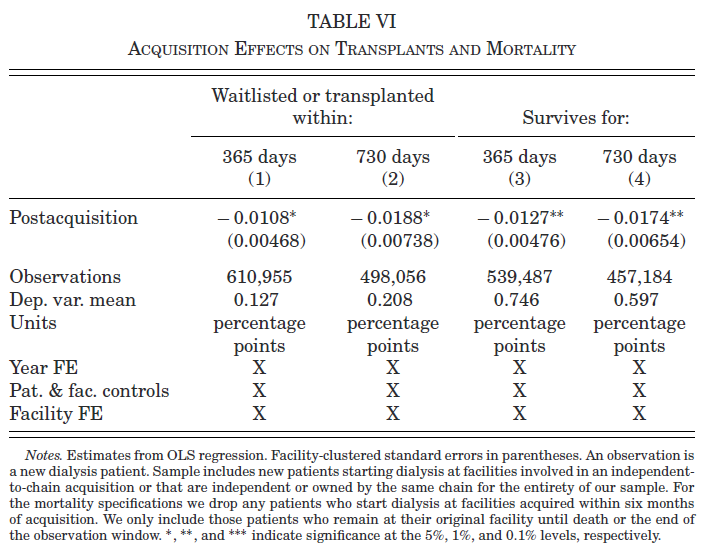
\includegraphics[width=90mm]{figure3_4.png}
        \label{fig:method}
        \end{figure}
        \vspace{-9.5mm}

\end{frame}

\begin{frame}{The Effect of Competition on Firm Behavior}

\begin{itemize}
\item With the price fixed by Medicare, facilities may compete for patients by offering higher-quality treatments.
\item Such competition may prevent the acquirer from implementing its strategy to increase profits.
\item To investigate the effect, define markets as hospital service areas (HSAs) and use a Herfindahl-Hirschman Index (HHI) to measure concentration.
\item Results show that market concentration does not mitigate the transference of firm strategy.
\item A key reason is that patients rarely respond to differences in quality.

\end{itemize}

\end{frame}

\begin{frame}\frametitle{Result: Acquisition Effect by Concentration}
\setlength{\leftmargini}{12pt}
\vspace{-7.5mm}
 \begin{figure}[h!]
        \centering
        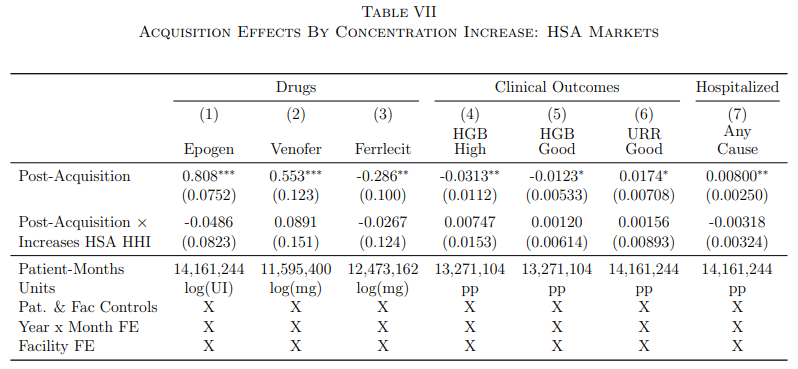
\includegraphics[width=130mm]{figure3_7.png}
        \label{fig:method}
        \end{figure}
        \vspace{-9.5mm}

\end{frame}

\begin{frame}\frametitle{Conclusion}
\setlength{\leftmargini}{12pt}

\begin{itemize}
    \item [1.] Acquisitions lead to clear changes in firm strategy that substantially worsen the quality of care received by patients and increase the cost of care borne by Medicare.
    \item [2.] Current antitrust statutes may do little to prevent the harmful effects of these acquisitions.
    \item [3.] Well-designed payment system is important for controlling health care costs and improving patient outcomes. 
    \begin{itemize}
        \item For example, the Quality Incentive Program initiated in 2012 allows Medicare to penalize providers that fail to meet certain quality standards.
    \end{itemize}
\end{itemize}


\end{frame}




\end{document}